\section{Dataset selection}
\label{chap:dataset}
The most complicated step to start with is to search for a dataset, it is the crucial part because a wrong dataset means a wrongly trained model, so searching for the dataset is important and takes a lot of time.
Being in fact so important I spent several hours to research, analyze different datasets, to finally find what I needed.
Initially for my work I chose the IMDb dataset, but not being ideal I then replaced it with the Hotel Review dataset. The problem with both datasets is that they are in English, and it turned out in the project that the articles to be analyzed would be only in German. I had to search for a dataset in German, and I found the Filmstarts one. Therefore, in the rest of the work, I will continue with the Filmstarts dataset.

\subsection{IMDB review description}
"Large Movie Review Dataset" \cite{noauthor_sentiment_nodate} is a dataset about movie reviews, consisting of 50k reviews which are divided into positive and negative reviews (no neutral).
This is a very famous and used dataset in the world of sentiment classification, other information can be found through the publication "Learning Word Vectors for Sentiment Analysis" \cite{maas-EtAl:2011:ACL-HLT2011}.

\subsubsection*{Motivation of the choice}
This dataset provides a categorization, i.e., it is a labelled dataset. Another advantage is that with \gls{Tensorflow} this dataset is particularly good for the methods I can use that we will see later.

\subsection{Hotel review description}
The dataset consists of approximately 515,000 customer reviews on over 1493 luxury hotels throughout Europe. Each review has a score ranging from 1 to 10. The dataset \cite{515k_kaggle} is hosted on \gls{kaggle} and is provided by Jiashen Liu.

\subsubsection*{Motivation of the choice}
The dataset provides an interesting set of datasets for sentiment analysis. These are provided with plenty of attributes. The structure of the datasets is kept very simple and understandable. Furthermore, \gls{kaggle} has rated this \gls{dataset} with a usability score of 8.2.

\subsection{Filmstarts description}
The Filmstarts dataset \cite{guhr_oliverguhrgerman-sentiment_2021} consists of 71,229 user written movie reviews in the German language. The dataset is a collection from the German website "filmstarts.de". The users can label their reviews in the range of 0.5 to 5 stars. With 40,049 documents the majority of the reviews in this data set are positive and only 15,610 reviews are negative.

\subsubsection*{Motivation of the choice}
The choice of this dataset fell on the German language, unfortunately there are not many datasets in this language. Fortunately having a score already made it easier to define a sentiment.

\section{Preprocessing the Filmstarts dataset}
\label{chap:work on dataset}
\subsection{Dataframe structure}
The dataset is a tab-separated values (TSV) file. A TSV file is a simple text format for storing data in a tabular structure.

First, I need to import the file using \gls{Pandas}, without importing lines with errors:

    \begin{tcolorbox}[breakable, size=fbox, boxrule=1pt, pad at break*=1mm,colback=cellbackground, colframe=cellborder]
\begin{Verbatim}[commandchars=\\\{\},fontsize=\footnotesize]
\PY{c+c1}{\PYZsh{} Load the data using \gls{Pandas}}
\PY{n}{film\PYZus{}de} \PY{o}{=} \PY{n}{pd}\PY{o}{.}\PY{n}{read\PYZus{}csv}\PY{p}{(}\PY{l+s+s2}{\PYZdq{}}\PY{l+s+s2}{filmstarts.tsv}\PY{l+s+s2}{\PYZdq{}}\PY{p}{,} \PY{n}{sep} \PY{o}{=} \PY{l+s+s1}{\PYZsq{}}\PY{l+s+se}{\PYZbs{}t}\PY{l+s+s1}{\PYZsq{}}\PY{p}{,}\PY{n}{encoding}\PY{o}{=}\PY{l+s+s1}{\PYZsq{}}\PY{l+s+s1}{utf8}\PY{l+s+s1}{\PYZsq{}}\PY{p}{,} \PY{n}{error\PYZus{}bad\PYZus{}lines}\PY{o}{=}\PY{k+kc}{False}\PY{p}{,} \PY{n}{warn\PYZus{}bad\PYZus{}lines}\PY{o}{=}\PY{k+kc}{True}\PY{p}{,} \PY{n}{header}\PY{o}{=}\PY{k+kc}{None}\PY{p}{)}
\end{Verbatim}
\end{tcolorbox}

The TSV file contains 3 columns, this means that one customer rating contains 3 attributes. In Table~\ref{tab:Dataframe structure F} all attributes are explained in detail:

\begin{longtable}[ c ]{| m{5cm} | m{8cm}|}
\hline
\multicolumn{2}{|c|}{\textbf{Dataframe structure}}                                                                                                         \\ \hline
\endfirsthead
%
\multicolumn{2}{c}%
{{\bfseries  Table \thetable\ continued from previous page}} \\
\hline
\multicolumn{2}{|c|}{\textbf{Dataframe structure}}                                                                                                         \\ \hline
\endhead
%
\textbf{ 0 }    & Url of the review.\\ \hline
\textbf{ 1 }    & Score Rating.\\ \hline
\textbf{ 2 }    & Text of the review.\\ \hline

\caption{Dataframe structure}
\label{tab:Dataframe structure F}\\
\end{longtable}

\subsection{Create an input and response dataframe}
I cleaned the dataframe to remove all the columns that I did not need.
After that I renamed the columns and reordered.
    \begin{tcolorbox}[breakable, size=fbox, boxrule=1pt, pad at break*=1mm,colback=cellbackground, colframe=cellborder]
\begin{Verbatim}[commandchars=\\\{\},fontsize=\small]
\PY{n}{film\PYZus{}de} \PY{o}{=} \PY{n}{film\PYZus{}de}\PY{o}{.}\PY{n}{rename}\PY{p}{(}\PY{n}{columns}\PY{o}{=}\PY{p}{\PYZob{}}\PY{l+m+mi}{2}\PY{p}{:} \PY{l+s+s1}{\PYZsq{}}\PY{l+s+s1}{Review}\PY{l+s+s1}{\PYZsq{}}\PY{p}{,} \PY{l+m+mi}{1}\PY{p}{:} \PY{l+s+s1}{\PYZsq{}}\PY{l+s+s1}{Score}\PY{l+s+s1}{\PYZsq{}}\PY{p}{\PYZcb{}}\PY{p}{)}
\end{Verbatim}
\end{tcolorbox}

            \begin{tcolorbox}[breakable, size=fbox, boxrule=.5pt, pad at break*=1mm, opacityfill=0]
\begin{Verbatim}[commandchars=\\\{\},fontsize=\footnotesize]
                                                  Review  Score
10                                    alle teile gemeint    0.0
11     ALSO:    Ich habe in meinem Leben schon viel S{\ldots}    0.0
55     der Vermarktung!     Ich frage mich allen Erns{\ldots}    1.0
58     Ey isch hab gestern Lordof the Weed gesehen ne{\ldots}    0.0
73     Also ich muss ehrlich sagen das ich es total l{\ldots}    1.0
{\ldots}                                                  {\ldots}    {\ldots}
71073  Zwei Stunden Lebenszeit vergeudet. Hier wird v{\ldots}    0.0
71078  Traumfrauen. Für viele von uns unerreichbar, e{\ldots}    1.0
71081  So einen drecks film sorry aber mir fällt leid{\ldots}    0.0

[7744 rows x 2 columns]
\end{Verbatim}
\end{tcolorbox}

Now that I have cleaned up the dataframes with what I needed, I see how they are composed, as can be seen from the chart in Figure~\ref{fig:fig_03} :

\begin{figure}[H]
\centering
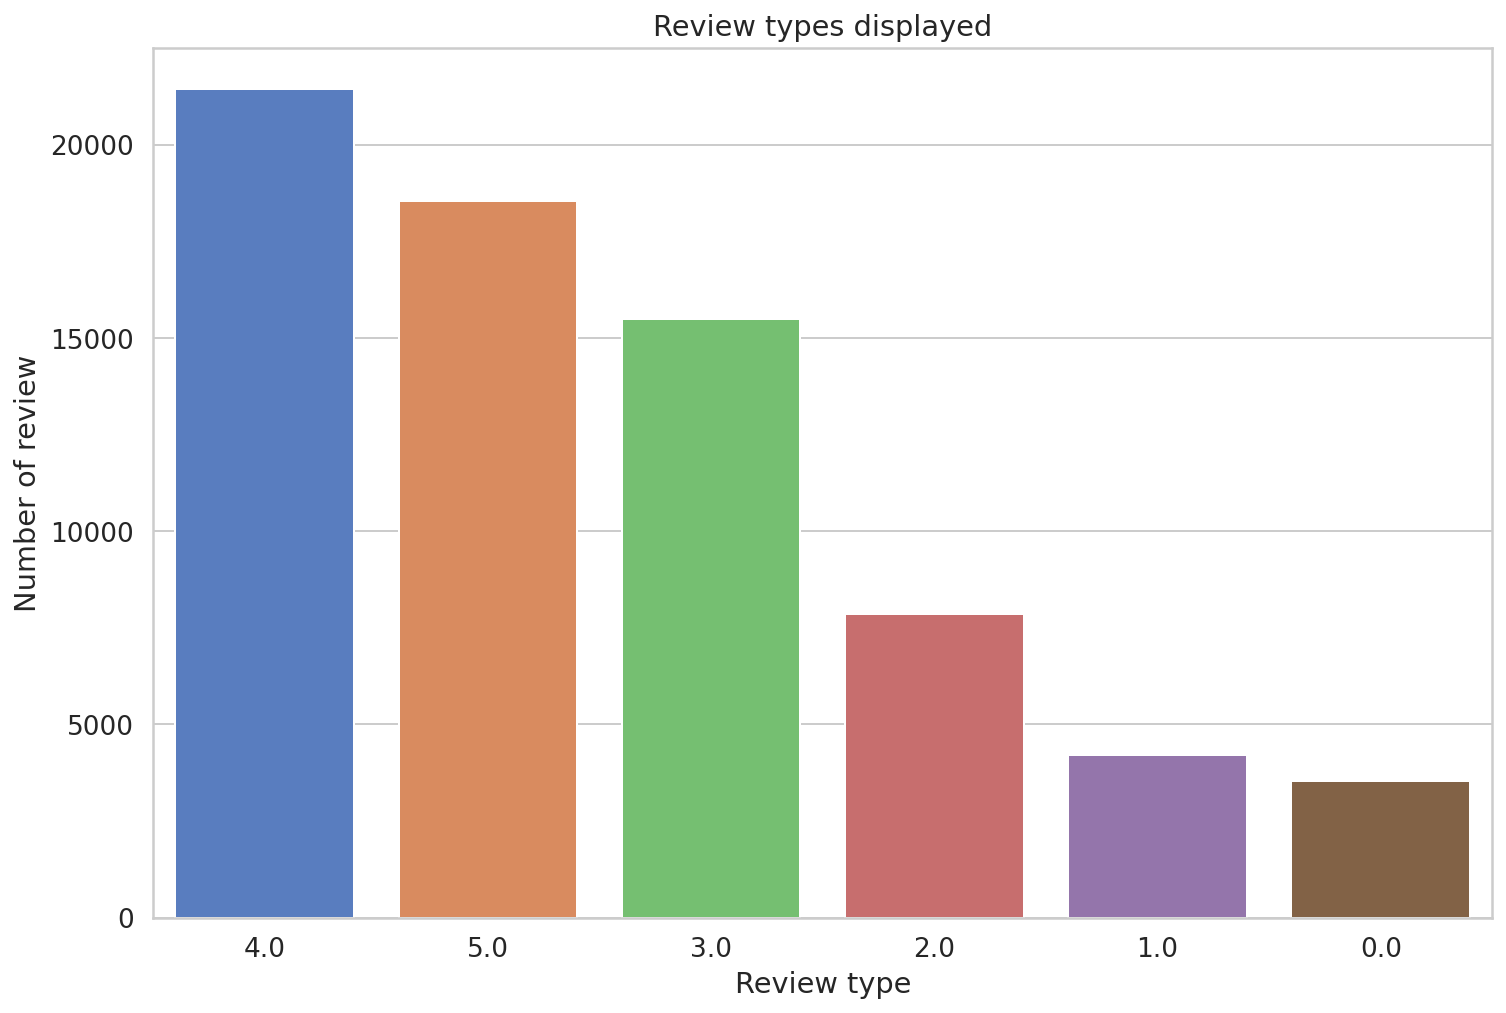
\includegraphics[width=1\textwidth]{images/output_37_1.png}
\caption{Number of ratings per category}
\label{fig:fig_03}
\end{figure}
\FloatBarrier


The "Polarity" of a review is determined by the following criteria:
\begin{itemize}
\item \textbf{"0"}: for the category with score 0.0
\item \textbf{"1"}: for the category with score 5.0
\end{itemize}
I did this to have only the worst and best reviews, so that I could have a clear distinction of words. And thus make it easier for the model to work.

The code for this operation is shown here below:

        \begin{tcolorbox}[breakable, size=fbox, boxrule=1pt, pad at break*=1mm,colback=cellbackground, colframe=cellborder]
\begin{Verbatim}[commandchars=\\\{\},fontsize=\footnotesize]
\PY{c+c1}{\PYZsh{} Get review type by aforementioned method}
\PY{k}{def} \PY{n+nf}{get\PYZus{}review\PYZus{}type}\PY{p}{(}\PY{n}{review\PYZus{}score}\PY{p}{)}\PY{p}{:}
    \PY{k}{if} \PY{n}{review\PYZus{}score} \PY{o}{\PYZlt{}}\PY{o}{=} \PY{l+m+mi}{0}\PY{p}{:}
        \PY{k}{return} \PY{l+m+mi}{0}
    \PY{k}{elif} \PY{n}{review\PYZus{}score} \PY{o}{\PYZgt{}}\PY{o}{=} \PY{l+m+mi}{5}\PY{p}{:}
        \PY{k}{return} \PY{l+m+mi}{1}
    \PY{k}{else}\PY{p}{:}
        \PY{k}{return} \PY{k+kc}{None}


\PY{n}{film\PYZus{}de}\PY{p}{[}\PY{l+s+s2}{\PYZdq{}}\PY{l+s+s2}{Positive}\PY{l+s+s2}{\PYZdq{}}\PY{p}{]} \PY{o}{=} \PY{n}{film\PYZus{}de}\PY{p}{[}\PY{l+s+s2}{\PYZdq{}}\PY{l+s+s2}{Score}\PY{l+s+s2}{\PYZdq{}}\PY{p}{]}\PY{o}{.}\PY{n}{apply}\PY{p}{(}
  \PY{k}{lambda} \PY{n}{x}\PY{p}{:} \PY{n}{get\PYZus{}review\PYZus{}type}\PY{p}{(}\PY{n}{x}\PY{p}{)}
\PY{p}{)}

\PY{c+c1}{\PYZsh{} Combine only the useful columns}
\PY{n}{film\PYZus{}df\PYZus{}de} \PY{o}{=} \PY{n}{film\PYZus{}de}\PY{p}{[}\PY{p}{[}\PY{l+s+s2}{\PYZdq{}}\PY{l+s+s2}{Review}\PY{l+s+s2}{\PYZdq{}}\PY{p}{,} \PY{l+s+s2}{\PYZdq{}}\PY{l+s+s2}{Positive}\PY{l+s+s2}{\PYZdq{}}\PY{p}{]}\PY{p}{]}
\end{Verbatim}
\end{tcolorbox}

Now we have the two categories 1 ("good") and 0 ("bad"). As can be seen from the chart in Figure~\ref{fig:fig_04}  the "good" category has many more values than the "bad" category.

\begin{figure}[H]
\centering
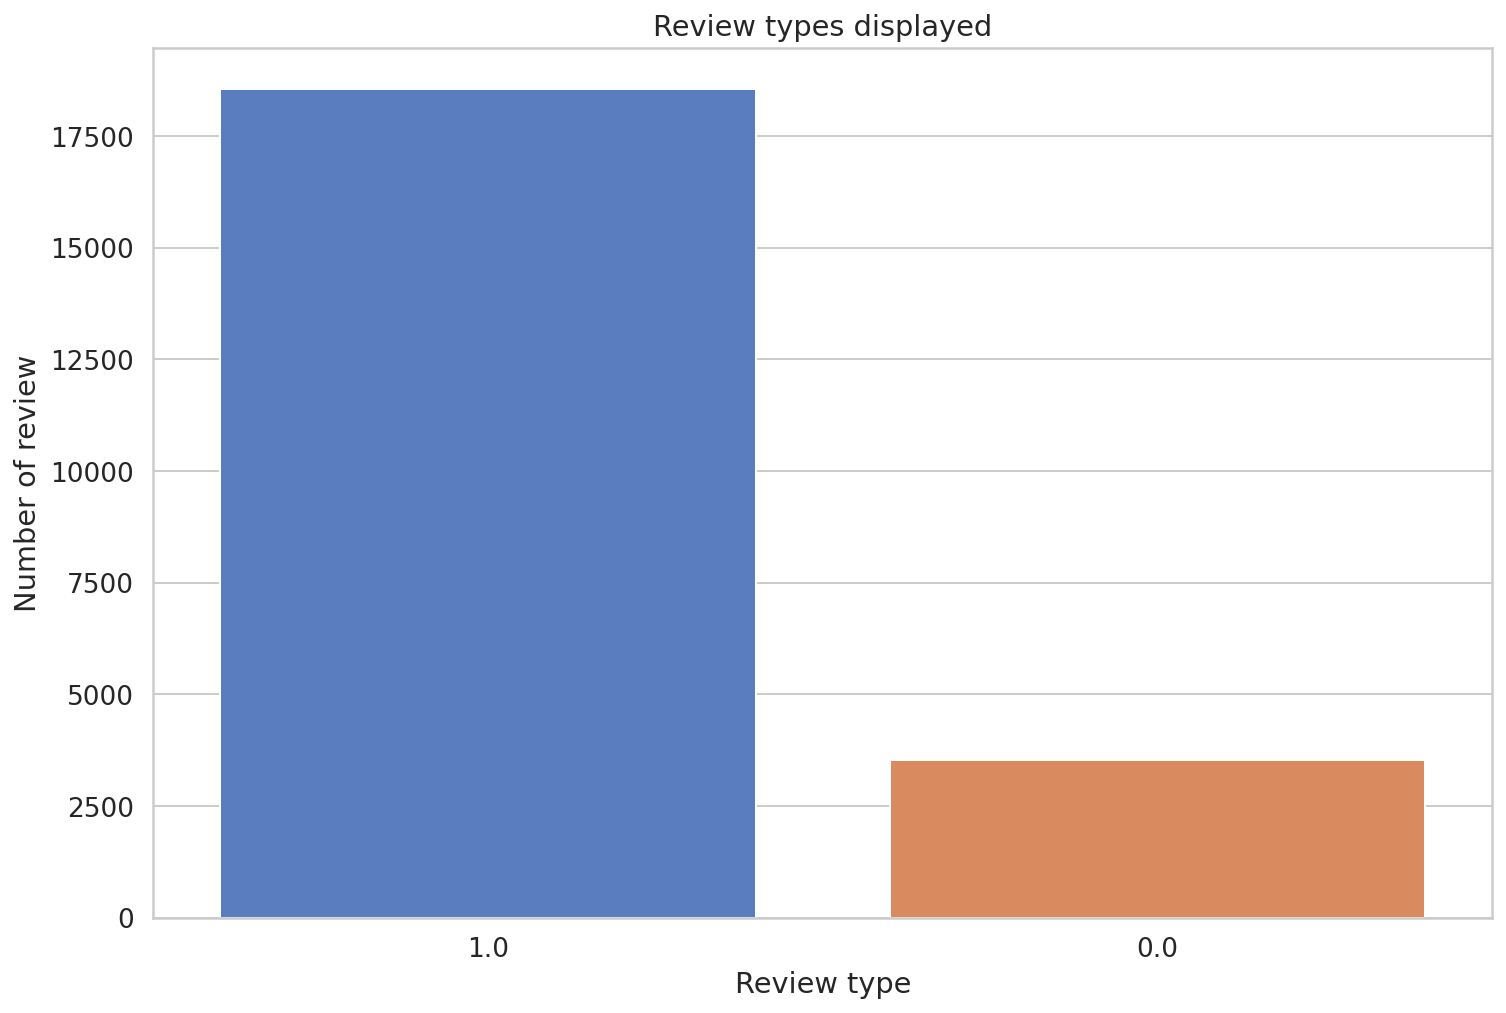
\includegraphics[width=1\textwidth]{images/output_43_1.png}
\caption{Number of ratings per category}
\label{fig:fig_04}
\end{figure}
\FloatBarrier
\subsection{Resample reviews}
\label{chap:resample}
In order to be able to train my model later on, I need to have the same amount of test data for each category. For this reason, I should limit the larger category to the value of the smaller one.
The code for this operation:
        \begin{tcolorbox}[breakable, size=fbox, boxrule=1pt, pad at break*=1mm,colback=cellbackground, colframe=cellborder]
\begin{Verbatim}[commandchars=\\\{\},fontsize=\footnotesize]
\PY{c+c1}{\PYZsh{} Get same number of reviews for each type}
\PY{n}{bad\PYZus{}reviews} \PY{o}{=} \PY{n}{film\PYZus{}df\PYZus{}de}\PY{p}{[}\PY{n}{film\PYZus{}df\PYZus{}de}\PY{o}{.}\PY{n}{Positive} \PY{o}{==} \PY{l+m+mi}{0}\PY{p}{]}
\PY{n}{good\PYZus{}reviews} \PY{o}{=} \PY{n}{film\PYZus{}df\PYZus{}de}\PY{p}{[}\PY{n}{film\PYZus{}df\PYZus{}de}\PY{o}{.}\PY{n}{Positive} \PY{o}{==} \PY{l+m+mi}{1}\PY{p}{]}

\PY{n}{sample\PYZus{}len} \PY{o}{=} \PY{n+nb}{len}\PY{p}{(}\PY{n}{bad\PYZus{}reviews}\PY{p}{)}

\PY{n}{bad\PYZus{}df} \PY{o}{=} \PY{n}{bad\PYZus{}reviews}
\PY{n}{good\PYZus{}df} \PY{o}{=} \PY{n}{good\PYZus{}reviews}\PY{o}{.}\PY{n}{sample}\PY{p}{(}\PY{n}{n}\PY{o}{=}\PY{n}{sample\PYZus{}len}\PY{p}{,} \PY{n}{random\PYZus{}state}\PY{o}{=}\PY{n}{RANDOM\PYZus{}SEED}\PY{p}{)}

\PY{n}{film\PYZus{}review\PYZus{}df} \PY{o}{=} \PY{n}{good\PYZus{}df}\PY{o}{.}\PY{n}{append}\PY{p}{(}\PY{n}{bad\PYZus{}df}\PY{p}{)}\PY{o}{.}\PY{n}{reset\PYZus{}index}\PY{p}{(}\PY{n}{drop}\PY{o}{=}\PY{k+kc}{True}\PY{p}{)}
\PY{n}{film\PYZus{}review\PYZus{}df}\PY{o}{.}\PY{n}{shape}
\end{Verbatim}
\end{tcolorbox}

By doing so, the data will have  the same number of entries as in Figure~\ref{fig:fig_05}.

\begin{figure}[H]
\centering
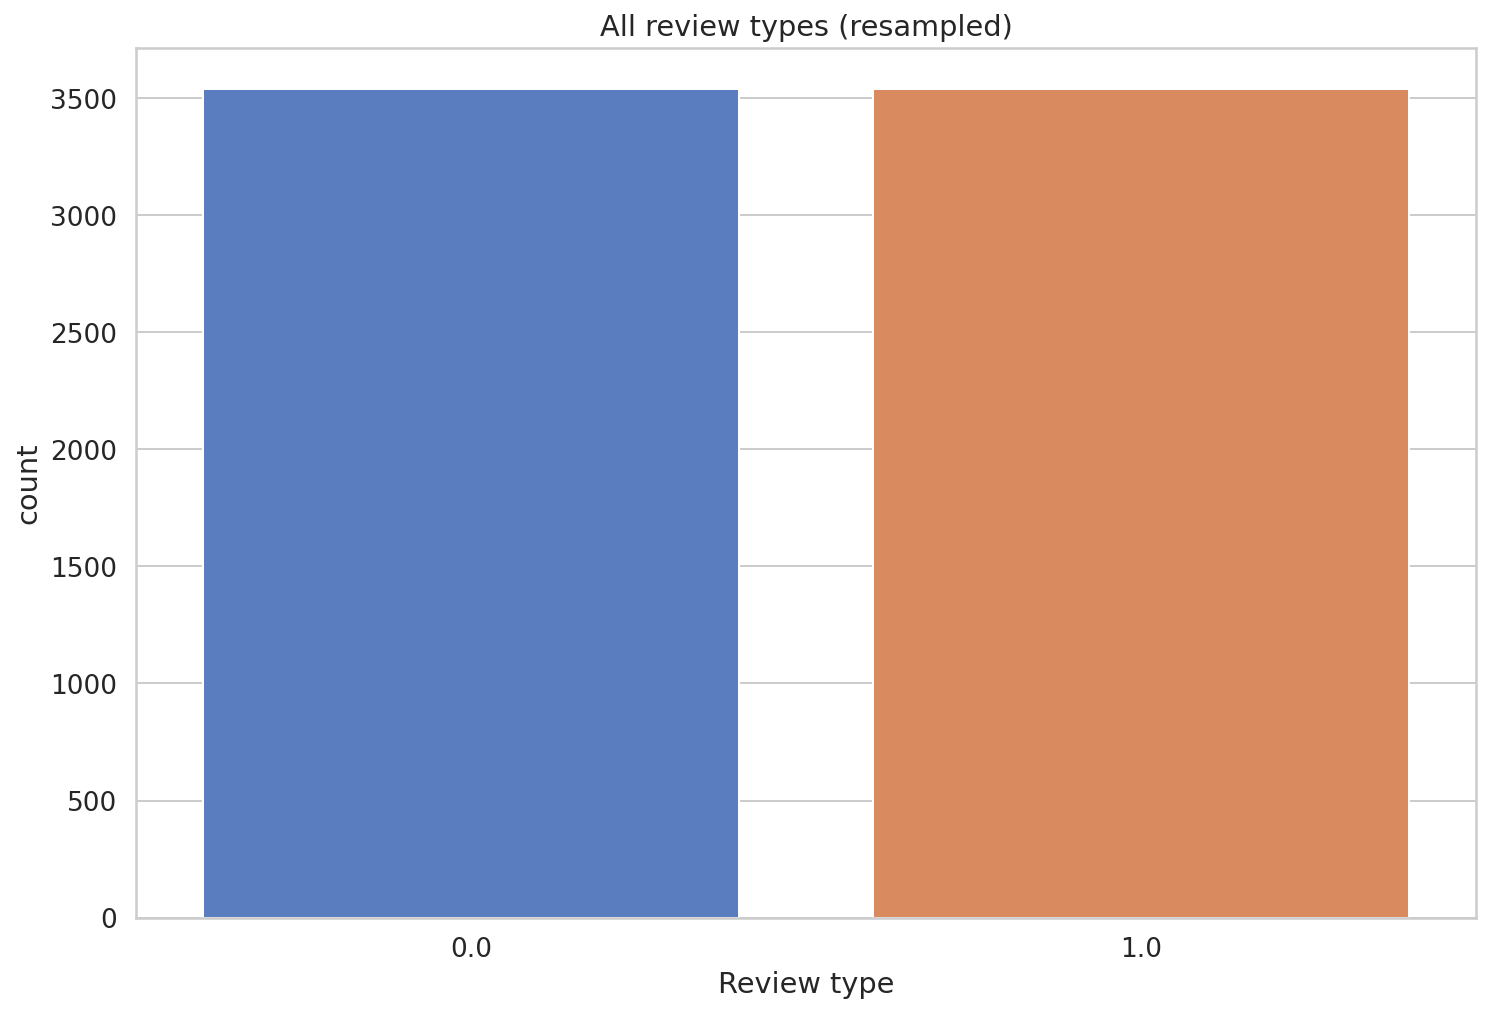
\includegraphics[width=1\textwidth]{images/output_47_0.png}
\caption{Uniform size of the categories}
\label{fig:fig_05}
\end{figure}
\FloatBarrier

\subsection{Preprocessing}
In this section I deal with the preparation of the data to give then to the model.
Before I start with splitting the dataset, I randomize the entire dataset by shuffling the data in a totally random way. 
The first thing to do is to split the dataframes I got after cleaning into 2 parts:
\begin{itemize}
    \item training set
    \item test set
\end{itemize}

Training set is a sample of data used to fit the model, the model trains and learns from this data.\\
Test set is used to evaluate the trained model. With the evaluation of the model, it is possible to make a fine-tune of the model and to modify the hyperparameters.\\
Real test data provides the gold standard used to evaluate the model.\\

Figure~\ref{fig:fig_06} shown an example of the split of a dataset\footnote{Reference figure \url{https://towardsdatascience.com/train-validation-and-test-sets-72cb40cba9e7}}: 
\begin{figure}[H]
\centering
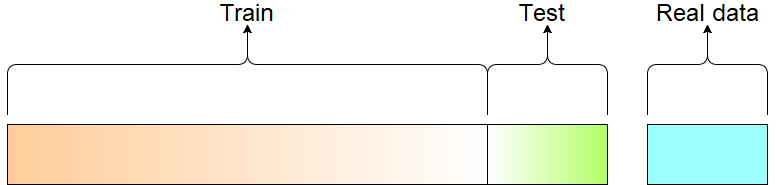
\includegraphics[width=1\textwidth]{images/traintestvali.jpg}
\caption{Data split}
\label{fig:fig_06}
\end{figure}
\FloatBarrier

Thanks to the library sklearn.model\_selection.train\_test\_split I can easily split my dataset in training and test. The division is done with a ratio 80\%(training)/20\%(test)

    \begin{tcolorbox}[breakable, size=fbox, boxrule=1pt, pad at break*=1mm,colback=cellbackground, colframe=cellborder]
\begin{Verbatim}[commandchars=\\\{\},fontsize=\small]
\PY{n}{train}\PY{p}{,} \PY{n}{test} \PY{o}{=} \PY{n}{train\PYZus{}test\PYZus{}split}\PY{p}{(}\PY{n}{film\PYZus{}review\PYZus{}df}\PY{p}{,}\PY{n}{test\PYZus{}size}\PY{o}{=}\PY{l+m+mf}{0.2}\PY{p}{)}
\end{Verbatim}
\end{tcolorbox}

   \begin{Verbatim}[commandchars=\\\{\},fontsize=\small]
size of training set: 5660
size of test set: 1416
    \end{Verbatim}

Finally, in order to have data that is usable by the \gls{Ktrain} library, I need to transform both sets into lists, and eliminate rows with null values.

Next I will use the real data from the journals, to do some testing. This test is to see, if with the real data the model behaves as it should. 